


\tikzset{every picture/.style={line width=0.75pt}} %set default line width to 0.75pt        

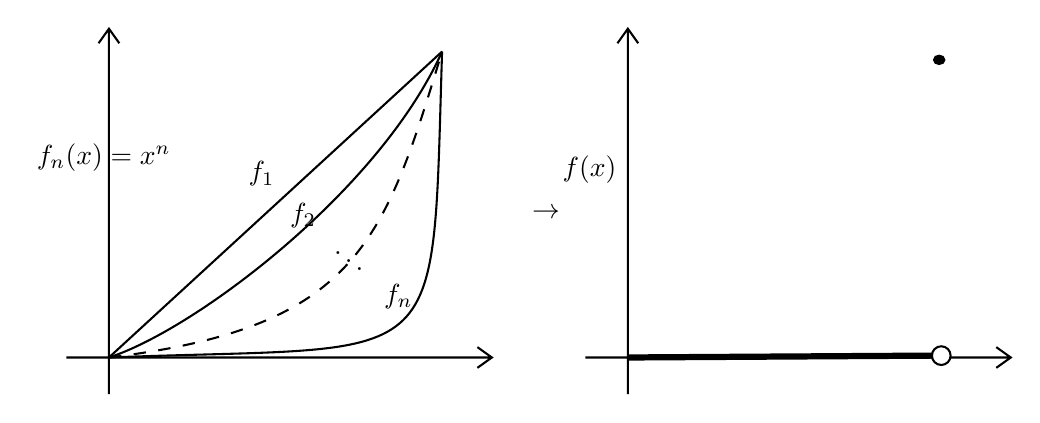
\begin{tikzpicture}[x=0.75pt,y=0.75pt,yscale=-1,xscale=1]
%uncomment if require: \path (0,478); %set diagram left start at 0, and has height of 478

%Shape: Axis 2D [id:dp905814360049316] 
\draw  (72,381.4) -- (277,381.4)(92.5,223) -- (92.5,399) (270,376.4) -- (277,381.4) -- (270,386.4) (87.5,230) -- (92.5,223) -- (97.5,230)  ;
%Shape: Axis 2D [id:dp0627612849597261] 
\draw  (322,381.4) -- (527,381.4)(342.5,223) -- (342.5,399) (520,376.4) -- (527,381.4) -- (520,386.4) (337.5,230) -- (342.5,223) -- (347.5,230)  ;
%Straight Lines [id:da2673655934702972] 
\draw    (92.5,381.4) -- (253,234) ;


%Straight Lines [id:da766634506285276] 
\draw [line width=2.25]    (342.5,381.4) -- (489,380.5) ;


%Shape: Ellipse [id:dp7944840513243177] 
\draw  [fill={rgb, 255:red, 0; green, 0; blue, 0 }  ,fill opacity=1 ] (490,238) .. controls (490,239.1) and (491.12,240) .. (492.5,240) .. controls (493.88,240) and (495,239.1) .. (495,238) .. controls (495,236.9) and (493.88,236) .. (492.5,236) .. controls (491.12,236) and (490,236.9) .. (490,238) -- cycle ;
%Shape: Circle [id:dp9726229856614172] 
\draw  [fill={rgb, 255:red, 255; green, 255; blue, 255 }  ,fill opacity=1 ] (489,380.5) .. controls (489,378.01) and (491.01,376) .. (493.5,376) .. controls (495.99,376) and (498,378.01) .. (498,380.5) .. controls (498,382.99) and (495.99,385) .. (493.5,385) .. controls (491.01,385) and (489,382.99) .. (489,380.5) -- cycle ;
%Curve Lines [id:da8879947029325801] 
\draw    (92.5,381.4) .. controls (134,368) and (223,301) .. (253,234) ;


%Curve Lines [id:da5540476052003762] 
\draw  [dash pattern={on 4.5pt off 4.5pt}]  (92.5,381.4) .. controls (212,367) and (225,326) .. (253,234) ;


%Curve Lines [id:da7987092769906381] 
\draw    (92.5,381.4) .. controls (257,375) and (248,393) .. (253,234) ;





% Text Node
\draw (90,285) node   {$f_{n}( x) =x^{n}$};
% Text Node
\draw (303,312) node   {$\rightarrow $};
% Text Node
\draw (166,293) node   {$f_{1}$};
% Text Node
\draw (186,313) node   {$f_{2}$};
% Text Node
\draw (232,352) node   {$f_{n}$};
% Text Node
\draw (208,331) node   {$\ddots $};
% Text Node
\draw (324,291) node   {$f( x)$};


\end{tikzpicture}
